\PassOptionsToPackage{style=phys}{biblatex}
\documentclass{beamer}

%%%% PACKAGES

\usepackage{import}
\usepackage[toc,page]{appendix}
\usepackage[T1]{fontenc}
\usepackage[english]{babel}
\usepackage[utf8]{inputenc}
\usepackage{graphicx}
\usepackage{adjmulticol}
\usepackage[labelfont=bf]{caption}
\usepackage{float}
\usepackage{graphicx}
\usepackage{subcaption}
\usepackage{fancyhdr}
\usepackage{url}
\usepackage{amsmath} % collection de symboles mathématiques
\usepackage{amssymb} % collection de symboles mathématiques
\usepackage{amsthm}
\usepackage{bbm}
\usepackage{bm}
\usepackage{stmaryrd}
\usepackage{mathtools}
\usepackage{cancel}
\usepackage{titling}
\usepackage{nameref} % pour désigner des parties par leur nom
\usepackage{url} % pour mettre des URL
\usepackage{cite}
% \usepackage[sectionbib]{chapterbib}
% \usepackage{chapterbib}
\usepackage[numbers,sort&compress]{natbib}
% \usepackage[square,numbers,sectionbib]{natbib}
% \usepackage{bibunits}
% \usepackage{biblatex}
\usepackage{tabularx}
\usepackage{titlesec, blindtext, color}
% \usepackage{auto-pst-pdf}

%%%% TIKZ

\usepackage{pgf, tikz}
\usetikzlibrary{shapes.misc}
\usetikzlibrary{decorations.pathreplacing}

\tikzset{cross/.style={cross out, draw=black, minimum size=2*(#1-\pgflinewidth), inner sep=0pt, outer sep=0pt},
%default radius will be 1pt.
cross/.default={0.25pt},
    point/.style={
    thick,
    draw=black,
    cross out,
    inner sep=0pt,
    minimum width=4pt,
    minimum height=4pt,
    },
}

%%%% STYLE

\textheight=25 true cm
\textwidth= 20. true cm
\oddsidemargin=-1.75truecm
\evensidemargin=0.5truecm
\topmargin=-3 truecm

% \setlength{\topmargin}{-1cm}
% \setlength{\headheight}{0.43cm}
% \setlength{\headsep}{0.8cm}
% \setlength{\footskip}{0cm}
% \setlength{\textwidth}{17cm}
% \setlength{\textheight}{23.5cm}
% \setlength{\voffset}{-2.5cm}
% \setlength{\hoffset}{-0.25cm}
% \setlength{\oddsidemargin}{0cm}
% \setlength{\evensidemargin}{0cm}
\setlength{\parindent}{0pt}
\setlength{\footskip}{1.5cm}

\setlength{\droptitle}{-1cm}

\setcounter{tocdepth}{3}
\setcounter{secnumdepth}{3}

\definecolor{lcolor}{rgb}{0,0,0.6} % définition de la couleur des liens pdf
\usepackage{hyperref}
\hypersetup{pdftex,colorlinks=true,
linkcolor=lcolor,
citecolor=lcolor,
urlcolor=lcolor,
hyperindex=true,
hyperfigures=false} % fichiers pdf 'intelligents', avec des liens entre les références, etc.

\definecolor{gray75}{gray}{0.75}

\AtBeginDocument{\addtocontents{toc}{\protect\thispagestyle{empty}}}

% \titleformat{\chapter}[hang]{\vspace{-50pt}\huge\bfseries}{\thechapter\hspace{20pt}\textcolor{gray75}{|}\hspace{20pt}}{0pt}{\huge\bfseries}
\titleformat{\subsection}[block]{\hspace{0em}}{\large\textbf\thesubsection}{1em}{\large\textbf}
\titleformat{\subsubsection}[block]{\hspace{0em}}{\Small\textbf\thesubsubsection}{1em}{\Small\textbf}

\usepackage{etoolbox}
\makeatletter
\patchcmd{\@chap@pppage}{\thispagestyle{plain}}{\thispagestyle{empty}}{}{}
\makeatother

\captionsetup{font=normalsize}
\captionsetup[sub]{font=scriptsize}

%%%% COMMANDS

\providecommand{\ie}{\textit{i.e.}~}

%\renewcommand*\thesection{\arabic{section}}

\makeatletter
\providecommand*\bigcdot{\mathpalette\bigcdot@{.5}}
\providecommand*\bigcdot@[2]{\mathbin{\vcenter{\hbox{\scalebox{#2}{$\m@th#1\bullet$}}}}}
\makeatother

\providecommand{\appropto}{\mathrel{\vcenter{
  \offinterlineskip\halign{\hfil$##$\cr
    \propto\cr\noalign{\kern2pt}\sim\cr\noalign{\kern-2pt}}}}}

\providecommand\encircle[1]{%
  \tikz[baseline=(X.base)]
    \node (X) [draw, shape=circle, inner sep=0] {\strut #1};}

\providecommand\phantomarrow[2]{%
  \setbox0=\hbox{$\displaystyle #1\to$}%
  \hbox to \wd0{%
    $#2\mapstochar
     \cleaders\hbox{$\mkern-1mu\relbar\mkern-3mu$}\hfill
     \mkern-7mu\rightarrow$}%
  \,}

\providecommand{\myparagraph}[1]{\paragraph{#1}\mbox{}\\\vspace{-5pt}}

\providecommand{\isEquivTo}[1]{\underset{#1}{\sim}}

\makeatletter
\providecommand{\subalign}[1]{%
  \vcenter{%
    \Let@ \restore@math@cr \default@tag
    \baselineskip\fontdimen10 \scriptfont\tw@
    \advance\baselineskip\fontdimen12 \scriptfont\tw@
    \lineskip\thr@@\fontdimen8 \scriptfont\thr@@
    \lineskiplimit\lineskip
    \ialign{\hfil$\m@th\scriptstyle##$&$\m@th\scriptstyle{}##$\crcr
      #1\crcr
    }%
  }
}
\makeatother

% \makeatletter
% % Original \l@section:
% %\renewcommand*\l@section{\vskip 6pt plus 1pt minus 1pt
% %                         \@dottedtocline{1}{1.5em}{2.3em}}
% % Modified \l@section:
% \renewcommand*\l@section{\ifnum\c@tocdepth>\z@\vskip 6pt plus 1pt minus 1pt \fi
%                          \@dottedtocline{1}{1.5em}{2.3em}}
% \makeatother

\providecommand\smallO[1]{
      \mathchoice
         {% mode \displaystyle
            \ensuremath{\mathop{}\mathopen{}{\scriptstyle\mathcal{O}}\mathopen{}\left(#1\right)}
         }
         {% mode \textstyle
            \ensuremath{\mathop{}\mathopen{}{\scriptstyle\mathcal{O}}\mathopen{}\left(#1\right)}
         }
         {% mode \scriptstyle
            \ensuremath{\mathop{}\mathopen{}{\scriptscriptstyle\mathcal{O}}\mathopen{}\left(#1\right)}
         }
         {% mode \scriptscriptstyle
            \ensuremath{\mathop{}\mathopen{}{o}\mathopen{}\left(#1\right)}
         }
   }

%%%% PATCH

% \makeatletter
% \let\orig@document\document
% \let\orig@enddocument\enddocument
% \def\sa@document{%
%   \endgroup
%   \global\let\enddocument\sa@enddocument
%   \sa@atbegindocument
% }
% \def\sa@enddocument{%
%   \sa@atenddocument
%   \global\let\document\orig@document
%   \global\let\enddocument\orig@enddocument
%   \begingroup
%   \@ignoretrue
%   \def\@currenvir{document}%
%   \aftergroup\endinput
% }
% \makeatother

\usepackage[mode=buildnew,subpreambles=true]{standalone}
\usepackage{cancel}
\usepackage{calc}
\usepackage{mdwlist}
\usepackage{xpatch}

%%%%% BEAMER TEMPLATE

\makeatletter
\let\insertsupervisor\relax
\renewcommand\supervisortitle{in collaboration with}
\mode<all>
{
  \renewcommand\supervisor[1]{\def\insertsupervisor{#1}}
  \titlegraphic{}
}
\makeatother

\AtEveryCitekey{\ifentrytype{article}{\clearfield{title}}{}}
\xpatchbibmacro{name:andothers}{%
  \bibstring{andothers}%
}{%
  \bibstring[\emph]{andothers}%
}{}{}
\setbeamercolor{bibliography entry author}{fg = black}
\ExecuteBibliographyOptions{doi=false}

%%%%% MACROS

\renewcommand{\FigureFrom}[2]{
  [{\usebeamercolor[fg]{caption source} from:} \fullcite{#1}\ifblank{#2}{}{ (Fig.~#2)}]
}

% https://tex.stackexchange.com/questions/199218
\usetikzlibrary{arrows,shapes}
\newcommand{\tikzmark}[2]{\tikz[baseline,remember picture]{\node[anchor=base] (#1){#2};}}

%%%%% CUSTOM COLOURS

% colorblind accessible palette ("red", "green", "blue", "yellow") contrasting with pink (#E85E8A)
% https://davidmathlogic.com/colorblind/#%23000000-%23E85E8A-%23CC78BC-%23D55E00-%230173B2-%23ECE133
\definecolor{red}{HTML}{CC78BC} % purple (#CC78BC)
\definecolor{green}{HTML}{029E73} % orange (#D55E00)
\definecolor{blue}{HTML}{0173B2} % blue (#0173B2)
\definecolor{yellow}{HTML}{ECE133} % yellow (#ECE133)

%%%%% INFORMATION

\title{Collective motion in large deviations of active particles}
\shorttitle{Large deviations of active particles (\href{https://doi.org/10.1103/PhysRevE.103.022603}{PRE \textbf{103}, 022603 (2021)})}

\author{Yann-Edwin Keta}

\location{APS March Meeting 2021}

\supervisor{E. Fodor, F. van Wijland, M.E. Cates, and R.L. Jack}

\date{19/03/2021}

%%%%% DOCUMENT

\begin{document}

%% TITLE PAGE AND OUTLINE

{
\setbeamertemplate{footline}{}
\makeatletter
    \setbeamertemplate{headline}[default]
    \def\beamer@entrycode{\vspace*{-\headheight}}
\begin{frame}[noframenumbering]

\vspace*{-4mm}
{
 \hspace*{-\beamerleftmargin}%
\begin{minipage}{\paperwidth}
\includegraphics[width=\paperwidth]{header.eps}
\end{minipage}
}

\titlepage

\vspace{-11.5pt}
\begin{center}
{\href{https://doi.org/10.1103/PhysRevE.103.022603}{Phys. Rev. E \textbf{103}, 022603 (2021)}}\\
\href{https://github.com/yketa/DAMTP_MSC_2019_Wiki}{\footnotesize \faGithub~ yketa/DAMTP\_MSC\_2019\_Wiki}
\end{center}

\vspace{-1pt}
\begin{center}
\begin{minipage}[c]{0.70\linewidth}
\includegraphics[height=0.75cm]{umontpellier.eps}
\hfill

\includegraphics[height=0.75cm]{cnrs.eps}
\hfill

\includegraphics[height=0.5625cm]{simons.eps}
\hfill
\includegraphics[height=0.75cm]{cambridge.eps}
\hfill

\includegraphics[height=0.75cm]{uparis.eps}
\end{minipage}
\end{center}

\end{frame}

}

{
\footerwithoutframenumber
\begin{frame}[noframenumbering]{Outline}

\begin{enumerate}
  \item Model of active Brownian particles.\\
  \return
  \item Active work and its large deviations.\\
  \return
  \item Description of dynamical phase transition.\\
  \return
  \item Mechanism for collective motion.
\end{enumerate}

\end{frame}
}

%% PRESENTATION

\begin{frame}[c]{Active Brownian particles model}

\footfullcitenomark{nemoto2019optimizing}
\footfullcitenomark{redner2013structure}

\begin{minipage}[c]{0.30\linewidth}
\begin{figure}
\centering
\includestandalone[width=0.85\textwidth]{abp}
\end{figure}
\end{minipage}
\hfill
\begin{minipage}[c]{0.65\linewidth}

\begin{center}
\bf standard ABP model
\end{center}
\begin{eqnarray}
&\dot{\boldsymbol{r}}_i = - D \nabla_i U(\{\boldsymbol{r}_j\}) + v_0 \boldsymbol{u}(\theta_i) + \sqrt{2 D} \boldsymbol{\eta}_i\\
&\dot{\theta}_i = \sqrt{2 D_r} \xi_i
\end{eqnarray}

\return
\begin{equation}
\tilde{l}_p = v_0 D_r^{-1} / \sigma
\end{equation}

\end{minipage}

\end{frame}

\begin{frame}{Active work}

\begin{center}
How far does the active forcing translate into real motion?
\end{center}

\pause
\begin{eqnarray}
% \text{EOM}& \dot{\boldsymbol{r}}_i = - D \nabla_i U + v_0 \boldsymbol{u}(\theta_i) + \sqrt{2 D} \boldsymbol{\eta}_i\\
% \text{dissipated power}& \dot{\mathcal{W}}_i = \sum_{i=1}^N \dot{\boldsymbol{r}}_i \circ \frac{1}{D} (\dot{\boldsymbol{r}}_i - \sqrt{2 D} \boldsymbol{\eta}_i)\\ \pause
% & \frac{1}{\tau} \int_0^{\tau} \dot{\mathcal{W}}_i(t) \, \mathrm{d}t \underset{\tau \to \infty}{=} \frac{N v_0^2}{D} {\color{CaPink} w_{\tau}}\\ \pause
\text{active work}& {\color{CaPink} w_{\tau}} = \frac{1}{v_0 N \tau} \sum_{i=1}^N \int_0^{\tau} \boldsymbol{u}(\theta_i) \circ \dot{\boldsymbol{r}}_i \, \mathrm{d}t
\end{eqnarray}
\pause

\return
\hfill
\begin{minipage}{0.4\linewidth}
\centering
\bf flocking
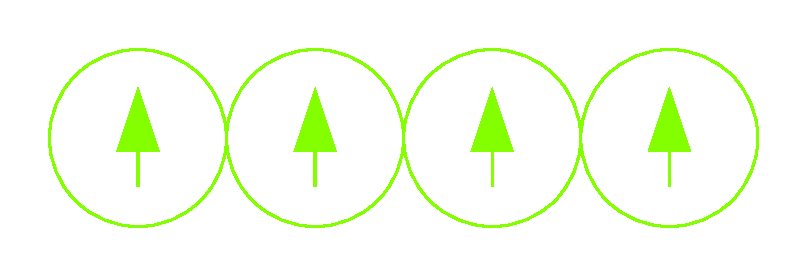
\includegraphics[width=\linewidth]{w1.eps}
$\dot{\boldsymbol{r}}_i \approx v_0 \boldsymbol{u}(\theta_i) \Rightarrow \left<{\color{CaPink} w_{\tau}}\right> = 1$
\end{minipage}
\hfill
\begin{minipage}{0.4\linewidth}
\centering
\bf jamming
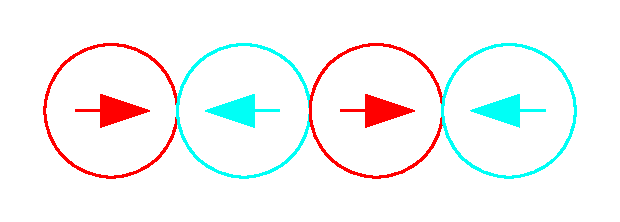
\includegraphics[width=\linewidth]{w0.eps}
$\dot{\boldsymbol{r}}_i \approx 0 \Rightarrow \left<{\color{CaPink} w_{\tau}}\right> = 0$
\end{minipage}
\hfill\hfill

\end{frame}

\begin{frame}{Large deviations}

\footfullcitenomark{touchette2009large}
\footfullcitenomark{jack2020ergodicity}
\footfullcitenomark{nemoto2016population}
\footfullcitenomark{cagnetta2017large}

\vspace{-15pt}
\begin{center}
How does the active work control emerging behaviours?
\end{center}
\vspace{-10pt}

\pause
\begin{equation}
P_s[\{\boldsymbol{r}_i, \theta_i\}_0^{\tau}] \propto P_0[\{\boldsymbol{r}_i, \theta_i\}_0^{\tau}] e^{-s N \tau {\color{CaPink} w_{\tau}}}
\end{equation}
\vspace{-5pt}

\pause
\begin{enumerate}
  \item Cloning algorithm $\Rightarrow$ trajectories biased with respect to $\color{CaPink} w_{\tau}$.
  \suspend{enumerate}
\pause
\begin{eqnarray}
& \left<\mathcal{A}\right>_s = \frac{\left<\mathcal{A}e^{-s N \tau {\color{CaPink} w_{\tau}}}\right>}{\left<e^{-s N \tau {\color{CaPink} w_{\tau}}}\right>}\\ \pause
& {\color{green} \psi}(s) = \lim_{\tau \to \infty} \frac{1}{N\tau} \log\left<e^{-s N \tau {\color{CaPink} w_{\tau}}}\right>
\end{eqnarray}
  \resume{enumerate}
  \pause
  \vspace{-5pt}
  \item Singularities in $\color{green} \psi$ $\Rightarrow$ qualitative changes at dynamical transition.
  \pause
  \item Compute probabilities of these fluctuations.
  \begin{eqnarray}
  & P({\color{CaPink} w_{\tau}}) \asymp \exp(-N \tau {\color{blue} I}({\color{CaPink} w_{\tau}}))\\
  & {\color{blue} I}({\color{CaPink} w_{\tau}}) = \sup_s \{-s {\color{CaPink} w_{\tau}} - {\color{green} \psi}(s)\}
  \end{eqnarray}
\end{enumerate}

% \begin{itemize}
%   \item[$\Rightarrow$] Cloning algorithm $\rightarrow$ generate trajectories of systems of ABPs where large deviations of the active work are typical.\pause
%   \begin{itemize}
%     \item[$\rightarrow$] Compute SCGF...
%     \begin{equation}
%       \psi_N(s, \tau) = \frac{1}{\tau} \log\left<e^{- s N \tau w_{\tau}}\right>,
%     \end{equation}
%     \begin{align*}
%       s > 0 \Leftrightarrow \text{large {\bf negative} fluctuations of } w(s)
%     \end{align*}
%     ... biased average of the active work...
%     \begin{equation}
%       w(s) = \left<w_{\tau}\right>_s = - \psi_N^{\prime}(s)/N,
%     \end{equation}
%     ... and rate function.
%     \begin{equation}
%       I_N(w) = \sup_s \left\{- s N w - \psi_N(s)\right\} = - s(w) N w - \psi_N(s(w)).
%     \end{equation}
%     \pause
%     \item[$\rightarrow$] Look for singularities in $I_N/N$ and $\psi_N/N$ $\Rightarrow$ fundamental changes in the mechanisms to produce the associated fluctuations of the active work.
%   \end{itemize}
% \end{itemize}

\end{frame}

\begin{frame}{Collective motion}

\footfullcitenomark{nemoto2019optimizing}

\begin{figure}
\begin{minipage}{0.48\linewidth}
\centering
unbiased steady state\\
$s = 0$
\Movie{1}{Nemoto_2019_unbiased.png}{Nemoto_2019_unbiased.mp4}
{\bf MIPS}
\end{minipage}
\hfill
\begin{minipage}{0.48\linewidth}
\centering
biased to large ${\color{CaPink} w_{\tau}}$\\
$s < 0$
\Movie{1}{Nemoto_2019_CM.png}{Nemoto_2019_CM.mp4}
{\bf CM}
\end{minipage}
\hfill\hfill
\end{figure}

\end{frame}

% \begin{frame}{Characterisation of the CM transition}
%
% \pause
% \begin{enumerate}[<+->]
%   \item Location $s^*$ of the transition.
%     \begin{equation}
%     s* \neq 0 \Rightarrow I \neq 0
%     \end{equation}
%   \item Mechanism of the transition.
% \end{enumerate}
%
% \end{frame}

\begin{frame}{CM transition point}

\footfullcitenomark{keta2021collective}

\vspace{-20pt}
\begin{center}
How much bias is needed for the transition to occur?
\end{center}
\pause

\vspace{-15pt}
% \begin{equation}
% \left<\mathcal{A}\right>_s = \frac{\left<\mathcal{A} e^{-s N \tau w_{f, \tau}}\right>_{v_s^{\rm con}}}{\left<e^{-s N \tau w_{f, \tau}}\right>_{v_s^{\rm con}}},~ v_s^{\rm con} = v_0 \left(1 - \frac{2 s D}{v_0^2}\right)
% \end{equation}
\begin{equation}
\boldsymbol{\nu} = \frac{1}{N} \sum_{i=1}^N \boldsymbol{u}(\theta_i),~ \bar{\nu}_{\tau} = \frac{1}{\tau} \int_0^{\tau} |\boldsymbol{\nu}(t)| \, \text{d}t
\end{equation}
\pause

\vspace{-5pt}
\begin{figure}
\centering
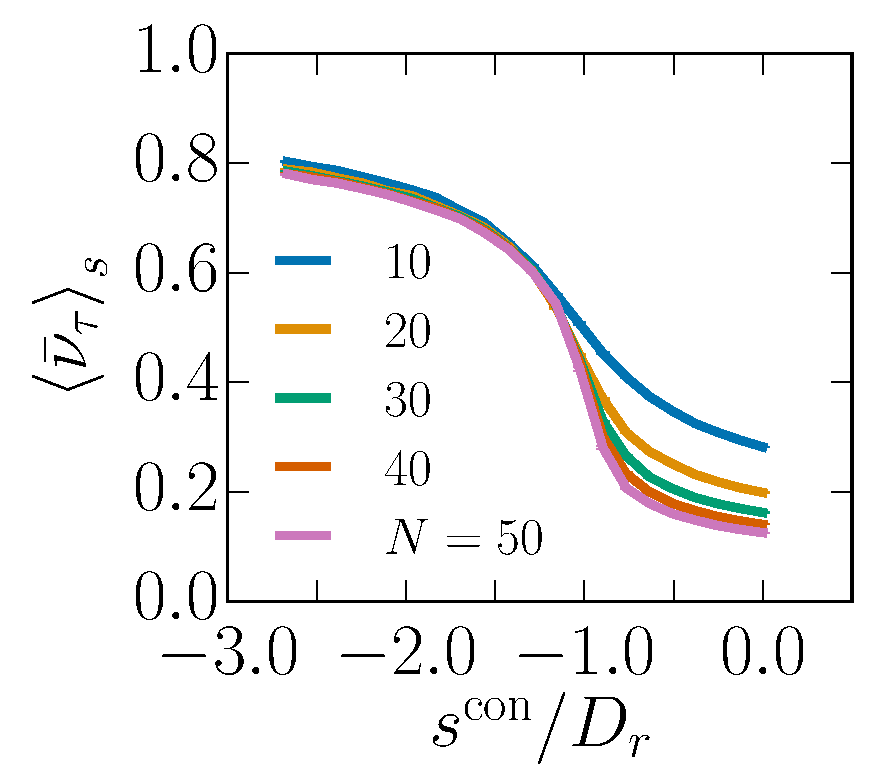
\includegraphics[width=0.45\textwidth]{sOrder_Dk6500_Ll5000_To1000-con.eps}
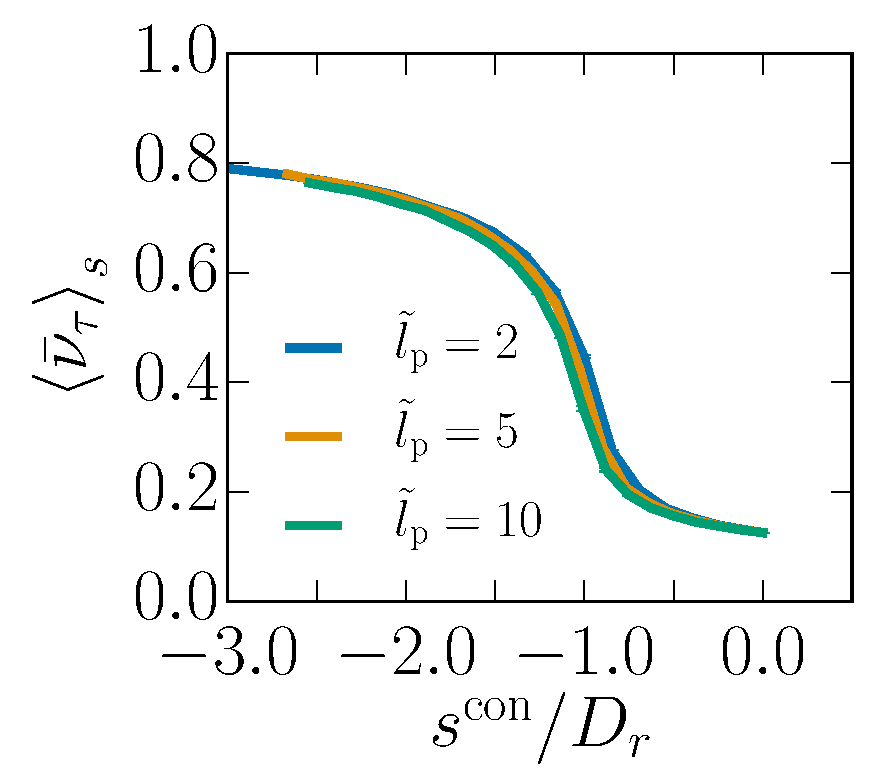
\includegraphics[width=0.45\textwidth]{sOrder_Nm5000_Dk6500_To1000-con.eps}
% \caption{{\bf (left)} Biased average of active work $\left<w_{\tau}\right>_s$. {\bf (right)} Biased average of global order parameter $\left<\bar{\nu}_{\tau}\right>_s$. $N=50$, $\phi = 0.65$.}
\end{figure}

\vspace{-20pt}
\pause
\begin{equation}
{s^{\rm con}}^* \approx -D_r
\end{equation}
\begin{center}
separation between steady state physics and symmetry breaking physics
\end{center}

% \pause
% \vspace{-5pt}
% \begin{equation}
% P(\left<{\color{CaPink} w_{\tau}}\right>_{s^*}) \asymp \exp(-N \tau {\color{blue} I}(\left<{\color{CaPink} w_{\tau}}\right>_{s^*}))
% \end{equation}

% \begin{itemize}
%   \item[$\rightarrow$] CM transition at finite $s^* \approx -D_r < 0$.
% \end{itemize}

\end{frame}

\begin{frame}{Modified dynamics}

\footfullcitenomark{den2008large}
\footfullcitenomark{jack2020ergodicity}
\footfullcitenomark{whitelam2018phase}
\footfullcitenomark{grandpre2021entropy}

\begin{center}
``Large deviations occur according to the least unlikely mechanism.''
\end{center}

\pause
\begin{eqnarray}
&\dot{\boldsymbol{r}}_i = - D \nabla_i U + v_0 \boldsymbol{u}(\theta_i) + \sqrt{2 D} \boldsymbol{\eta}_i\\
&\dot{\theta}_i = {\color{red}- D_r \frac{\partial}{\partial \theta_i} U^{\rm mod}_g} + \sqrt{2 D_r} \xi_i\\ \pause
&{\color{red} U_g^{\rm mod}} = - {\color{red} g} \frac{N |\boldsymbol{\nu}|^2}{D_r}
\end{eqnarray}

\pause
% \begin{itemize}
%   \item[$\Rightarrow$] Upper bound to the rate function.
% \end{itemize}

\begin{equation}
{\color{blue} I}({\color{CaPink} w}) \leq \lim_{\tau \to \infty} \mathcal{D}_{\rm KL}(P^{\rm mod}_{{\color{red} g}({\color{CaPink} w})} || P)
\end{equation}

\end{frame}

% \begin{frame}{Contraction principle}
%
% \footfullcitenomark{nemoto2019optimizing}
%
% % \begin{itemize}
% %   \item[$\rightarrow$] Since probabilities are measured on the exponential scale, the probability of any large fluctuation should be approximated by the probability of the least improbable event leading to this fluctuation.
% % \end{itemize}
% \begin{equation}
% {\color{blue} I}_{h(A)}(b) = \inf_{a:h(a)=b} {\color{blue} I}_A(a)
% \end{equation}
%
% \pause
% \return
% % \begin{itemize}
% %   \item[$\Rightarrow$] Lower bound to the rate function.
% % \end{itemize}
%
% % \begin{eqnarray}
% % \text{polarisation rate function}& &J(\nu)\\
% % \text{joint rate function}& &I_2(w, \nu)
% % \end{eqnarray}
%
% \begin{equation}
% \nu \equiv \bar{\nu}_{\tau} = \frac{1}{\tau} \int_0^{\tau} \hat{\nu}(t) \, \text{d}t
% \end{equation}
% \begin{equation}
% {\color{blue} I}({\color{CaPink} w}) \only<2->{{\color{red} \underset{\rm CP}{=}} \inf_{\nu} I_2({\color{CaPink} w}, \nu) \only<3->{= I_2({\color{CaPink} w}, \nu({\color{CaPink} w})) \only<4->{\boldsymbol{{\color{blue}\geq}} \inf_{w^{\prime}} I_2(w^{\prime}, \nu({\color{CaPink} w}))  \only<5->{{\color{red} \underset{\rm CP}{=}} {\color{blue} \mathcal{J}_1}(\nu({\color{CaPink} w}))}}}}
% \end{equation}
% % \return
% % \begin{equation}
% % {\color{blue} I(w)} {\color{red} \underset{\rm CP}{=}} \inf_{\nu} I_2(w, \nu) = I_2(w, \nu(w)) {\color{blue}\geq} \inf_{w^{\prime}} I_2(w^{\prime}, \nu(w)) {\color{red} \underset{\rm CP}{=}} {\color{blue} \mathcal{J}_1(\nu(w))}
% % \end{equation}
% \pause\pause\pause
%
% \end{frame}

\begin{frame}{Bounds to the rate function}

\footfullcitenomark{keta2021collective}

\begin{figure}
\includegraphics[height=5cm]{boundRate40.eps}
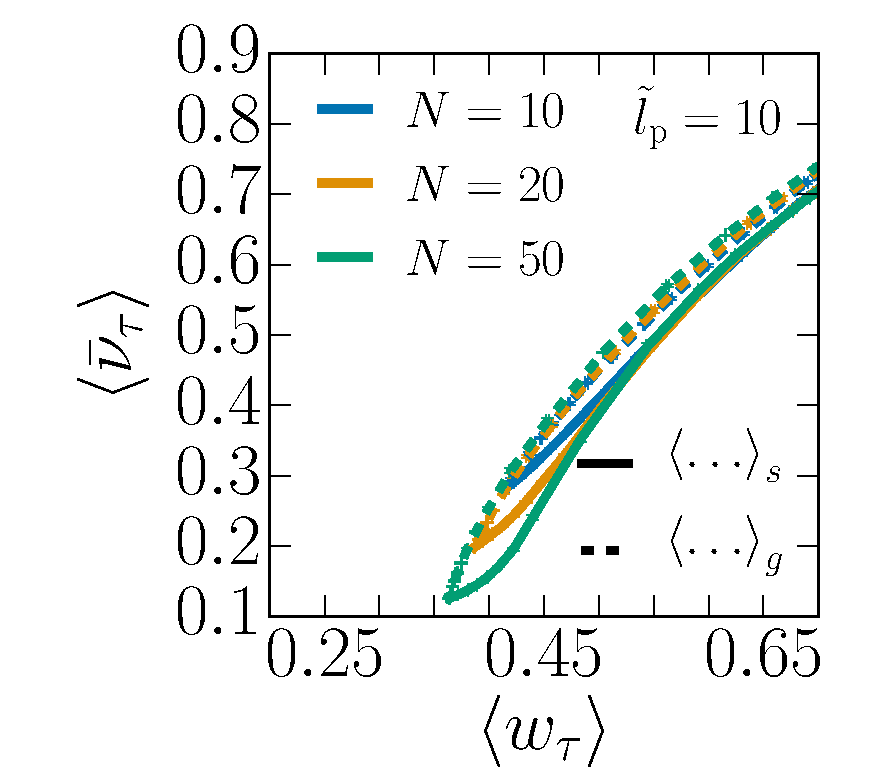
\includegraphics[height=5cm]{nuW_Lm1000.eps}
\end{figure}

\pause
\begin{center}
CM: fluctuations of ${\color{CaPink} w_{\tau}}$ strongly coupled to those of $\bar{\nu}_{\tau}$
\end{center}

\pause
\begin{center}
CM: response to biasing $s$ $\leftrightarrow$ response to aligning interaction $g$
\end{center}

\end{frame}

\begin{frame}[t]{Conclusion}

\pause
\begin{itemize}[<+->]
  \item We have introduced a model of {\bf active Brownian particles} biased with respect to a measure of the {\bf active work} ${\color{CaPink} w_{\tau}}$.
  \item This model of isotropic active matter displays {\bf collective motion} (CM) when ${\color{CaPink} w_{\tau}}$ is increased ($s < 0$).
  \item This transition to CM happens at {\bf finite biasing} $s^* \sim -D_r$ implying that these fluctuations are very distinct from the unbiased behaviour.
  \item It is qualitatively understood through the introduction of {\bf effective aligning interaction}.
  \item[]
  \begin{center}
  \centering \fbox{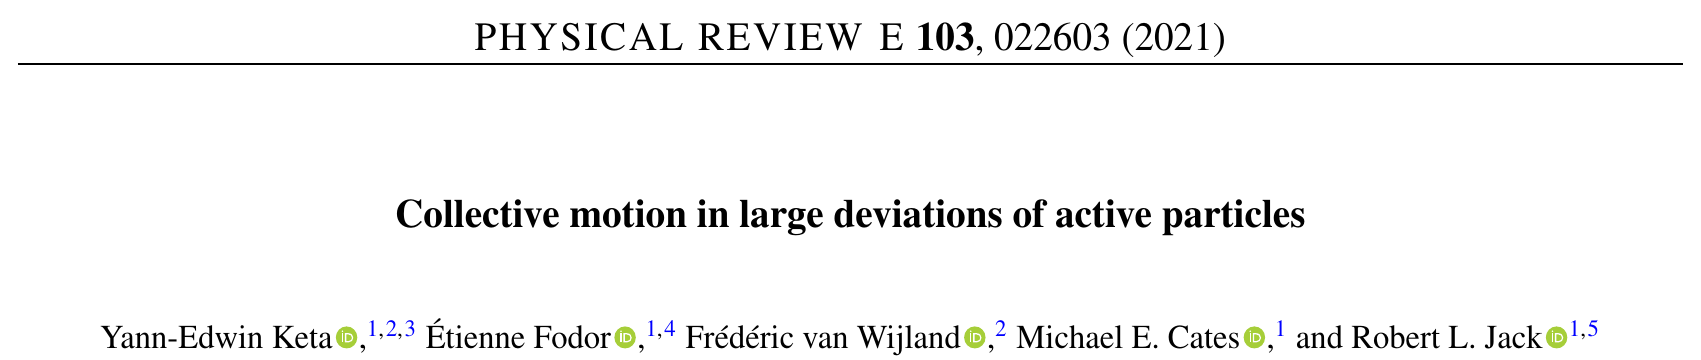
\includegraphics[width=0.80\linewidth]{header_paper.png}}
  \end{center}
  \item We compute exactly for a system of {\bf 2 particles on a ring} the relation between ${\color{CaPink} w_{\tau}}$ and particle alignment.
  \item We propose a {\bf fluctuating hydrodynamic theory} which captures the emergence of polar order in the biased state.
\end{itemize}

\end{frame}

%% THANK YOU

{
\footerwithoutframenumber
\begin{frame}[noframenumbering]

\begin{center}
\Huge
Thank you!
\end{center}

\end{frame}
}

%% SUPPLEMENTAL FRAMES

{
\footerwithoutframenumber

\begin{frame}[noframenumbering]{Suppression of density fluctuations}

\footfullcitenomark{dolezal2019large}

\vspace{-15pt}
\begin{itemize}
  \item At $\boldsymbol{P} = 0$, biasing w.r.t. $w_{\tau}$ is equivalent to biasing w.r.t. $|\tilde{\rho}_{\boldsymbol{q}}|^2$.
\end{itemize}

\begin{equation}
S_s(\boldsymbol{q}) = \left<|\tilde{\rho}_{\boldsymbol{q}}|^2\right>_s = \begin{cases} \chi_0, &s = 0 \\ b_s q, &s < 0 \end{cases}
\end{equation}
\begin{itemize}
  \item[$\Rightarrow$] We expect hyperuniformity in the isotropic $s < 0$ phase for $N \gg 1$.
\end{itemize}

\begin{figure}
\centering
\includegraphics[width=0.5\textwidth]{S_Nn1000_Dk6500_Ll5000_NCo1000.eps}
\caption{Biased structure factor $S_s$.}
\end{figure}

\vspace{-10pt}
\begin{itemize}
  \item[$\rightarrow$] Finite system shows suppression of density fluctuations for $s < 0$.
\end{itemize}

\end{frame}

}

\end{document}
